\documentclass[tikz,convert={density=150,size=600,outext=.png}]{standalone}
\usetikzlibrary{shapes, calc, arrows, fit, positioning, decorations, patterns, decorations.pathreplacing, chains, snakes}

\begin{document}
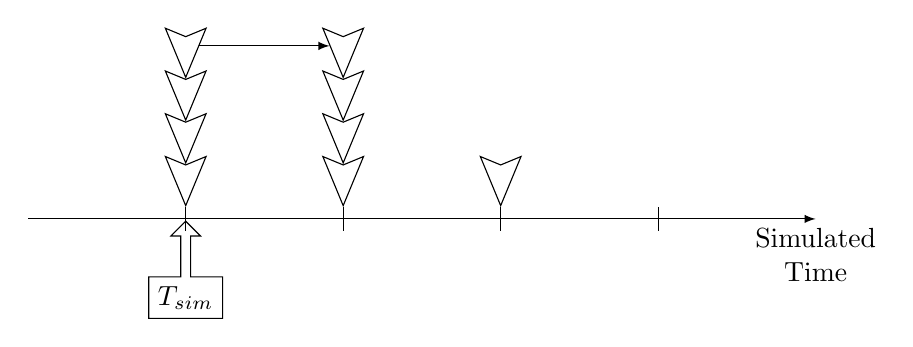
\begin{tikzpicture}[>=latex, node distance=0cm]
    \draw[->] (0,0) -- (10,0) node[pos=1, below, align=center] (sim-time1) {Simulated\\Time};
    \foreach \x in { 1, 2, 3, 4 } {
        \draw (\x*2,-0.15) -- (\x*2,0.15) node (tick\x) {};
    };

    \node[draw, arrow box, arrow box arrows={north:.7cm}] at (2, -1) {$T_{sim}$};

    \node[shape=dart, draw, , shape border rotate=270, above=of tick1.center] (ev11) {};
    \node[shape=dart, draw, , shape border rotate=270, above=of ev11.north] (ev12) {};
    \node[shape=dart, draw, , shape border rotate=270, above=of ev12.north] (ev13) {};
    \node[shape=dart, draw, , shape border rotate=270, above=of ev13.north] (ev14) {};

    \node[shape=dart, draw, , shape border rotate=270, above=of tick2.center] (ev21) {};
    \node[shape=dart, draw, , shape border rotate=270, above=of ev21.north] (ev22) {};
    \node[shape=dart, draw, , shape border rotate=270, above=of ev22.north] (ev23) {};
    \node[shape=dart, draw, , shape border rotate=270, above=of ev23.north] (ev24) {};

    \node[shape=dart, draw, , shape border rotate=270, above=of tick3.center] (ev31) {};

    \draw[->] (ev14) -- (ev24);
    \end{tikzpicture}
\end{document}
